\section{Theory Behind The GranFilm Software}
%To understand the theoretical background behind GranFilm and scattering on diffuse surfaces, it is 
%convenient to start with the simple case of scattering on a flat interface of two different half-infinite
%media, see Figure !!FIGUREREF HERE!!.
This section recapitulate the theoretical background behind GranFilm, a software used to calculate
the optical properties of granular thin films. 
\subsection{Theoretical Introduction; Flat Surface Scattering} \label{sectionFlatScattering}
Starting from basic electromagnetic theory, the simplest case 
of electromagnetic scattering is the transmission and reflection of light, hitting a flat,
smooth interface between two different half-infinite media. 
The electric permittivity $\varepsilon$ and magnetic permeability $\mu$ of the media are given 
with subscript $+$ for the upper media, and $-$ for the lower media, see Figure \ref{fig:flatScattering}. 
\begin{figure}[h!]
  \centering
   \includegraphics[width=1.0\textwidth]{Figures/flatSurfaceScattering.pdf}
   \caption{The reflection and transmission of an incident electromagnetic plane wave on a flat interface
      between two media. The dielectric functions for the upper and lower media are $\varepsilon_{+}(\omega)$
      and  $\varepsilon_{-}(\omega)$, respectively. The polarization direction $\boldsymbol{p}$ is the
      polarization parallel to or inside the place of incidence, while $\boldsymbol{s}$, which comes from the
      german word \textit{senkrecht} meaning perpendicular, is the perpendicular polarization.
      The figure is adopted from (\cite{Lazzari2002}, p.125).
   }
   \label{fig:flatScattering}
\end{figure}
Assuming that the incoming electromagnetic wave is a plane wave, the reflection and transmission
of the wave can be calculated from Maxwell's equations,
%
\begin{subequations}
\label{ME}
\begin{align}
   \nabla \cdot \boldsymbol{D} &= \rho \!_f           &\nabla\times\boldsymbol{E} &= - \frac{\partial \boldsymbol{B}}{\partial t} \label{ME1}\\
   \nabla \cdot \boldsymbol{B} &= 0                &\nabla \times \boldsymbol{H}&= \boldsymbol{J}\!_f + \frac{\partial \boldsymbol{D}}{\partial t}, \label{ME2}
\end{align}
\end{subequations}
%
which describe the general behavior of electromagnetic waves.
Here the electric field $\boldsymbol{E}$, the electric displacement $\boldsymbol{D}$,
the magnetic field $\boldsymbol{H}$ and the magnetic induction $\boldsymbol{B}$
are pairwise related through
\begin{align}
   \label{linearConstitutiveRelations}
   &\boldsymbol{D} = \varepsilon \boldsymbol{E},         &\boldsymbol{H} = \frac{1}{\mu} \boldsymbol{B}
\end{align}
(assuming linear media) (\cite{Griffiths}, p.330). 
Further assuming that there
is no free charge or free current at the interface, Maxwell's equation provide the boundary conditions 
(\cite{Griffiths}, p.333)
%
\begin{subequations}
\label{BC}
\begin{align}
   D^+_{\perp} &= D^-_{\perp}      &\boldsymbol{E}^+_{\parallel} = \boldsymbol{E}^-_{\parallel} \label{BC1}\\
   B^+_{\perp} &= B^-_{\perp}      &\boldsymbol{H}^+_{\parallel} = \boldsymbol{H}^-_{\parallel}. \label{BC2}
\end{align}
\end{subequations}
%
($\perp$ and $\parallel$ denotes the perpendicular and parallel komponent with respect to the 
surface boundary. By enforcing these boundary conditions on the incident, reflected and transmitted 
waves, on the entire boundary, the reflection and transmission coefficients may be calculated. The 
coefficients are given by
\begin{align}
   R &\equiv \frac{I_r}{I_i}     &T &\equiv \frac{I_t}{I_i}, \label{refTransCoeffs1}\\
\end{align}
where $I_x, x \in [i,r,t]$ is the intensity or power per unit area stricking/leaving the interface
for the incident, reflected and transmitted light, respectively (\cite{Griffiths},p.386-391).
The calculation can be found in any standard optics textbook \textit{NEED OPTICS BOOK REFERENCE}
and gives
\begin{align}
   R &= r^2       &T &= \frac{n\!_{_-} \cos \theta_t}{n\!_{_+} \cos \theta _i}. \label{refTransCoeffs2}\\
\end{align}
$n\!_{_+}$ and $n\!_{_-}$ are the indices of refraction for the media above (+) and belov (-) the interface,
while $\theta_i$ and $\theta_t$ gives the incident and transmitted lights direction with respect to the 
surface normal. 
The coefficients $r$ and $t$ are called the Frensel coefficients and their values depend on the
polarization of the incident light. For the flat interface the coefficients take the form
\textit{NEED ANOTHER OPTICS BOOK REFERENCE}
%
\begin{subequations}
\label{flatFresnelCoeff}
\begin{align}
   r_s &= \frac{n\!_{_+} \cos \theta_i - n\!_{_-} \cos \theta_t}
   {n\!_{_+} \cos \theta_i + n\!_{_-} \cos \theta_t}     
   &t_s &= \frac{2 n\!_{_+} \cos \theta_i}
   {n\!_{_+} \cos \theta_i + n\!_{_-} \cos \theta_t}, \label{flatFresnelCoeffs} \\
%
   r_p &= \frac{n\!_{_-} \cos \theta_i - n\!_{_+} \cos \theta_t}
   {n\!_{_+} \cos \theta_t + n\!_{_-} \cos \theta_i}     
   &t_p &= \frac{2 n\!_{_+} \cos \theta_i}
   {n\!_{_+} \cos \theta_t + n\!_{_-} \cos \theta_i}     \label{flatFresnelCoeffp}
\end{align}
\end{subequations}
%
so the reflection and transmission are different 
for the two polarization directions, which can be seen in Figure \ref{fig:flatScattering}.

\subsection{Scattering On Rough Surfaces: Excess Fields And Surface Susceptibilities}
When moving away from a flat surface, looking at a more complicated geometry of the boundary 
between the two media, the behavior of the dielectric function gets correspondingly diffucult.
Situations like these might be encountered for rough surfaces or granular thin films, where the latter
means that a foreign material is distributed as small island on top of a substrate. 
In these situations the calculation of the Fresnel coefficients turns increasingly complex (\cite{Lazzari2002},p.125).
\\
\\
However, in order to calculate such complicated surfaces, 
Bedeaux and Vlieger (\cite{Lazzari2002}, (7-12)) developed an approach in which the exact knowledge
of the electromagnetic fields close to the surface is not required. Their formalism is based on the notion 
of excess quantities. 
The excess fields are defined as the differene between the real fields and the bulk fields extrapolated
to the surface, where the bulk field simply means the field given sufficiently far away from the
scattering surface. E.g. for the electric field $E(r)$ the excess quantity is defined as
%
\begin{align}
   \label{excessField1}
   \boldsymbol{E}_{ex} (\boldsymbol{r}) \:=\: \boldsymbol{E}(\boldsymbol{r}) 
   \:-\: \boldsymbol{E}^-(\boldsymbol{r})\theta(-z) \:-\: \boldsymbol{E}^+(\boldsymbol{r})\theta(z),
\end{align}
%
where $\theta(z)$ is the Heaviside function and the superscript $\pm$ are used to indicate the region
above (+) and below (-) the dividing interface at $z = 0$. In addition, the optical frequency $\omega$
is implicitly included in the notation. Furthermore, the excess field is only significant close
to the surface, since $\boldsymbol{E}(\boldsymbol{r},\omega) \rightarrow 
\boldsymbol{E}^{\pm}(\boldsymbol{r},\omega)$ when $z \rightarrow \pm \infty$. \\
\textit{???is this correct???}
By integrating these excess fields along the z-axis, which is set normal to the surface,
%
\begin{subequations}
\label{intExQuant} % integrated excess quantities
\begin{align}
   \boldsymbol{D}^s_{\parallel}(\boldsymbol{r}) &= \!\!\!\!\!\!\!\!\! \int\limits ^{\:\:\:\:\:\:\:\:\:\:+\infty}_{\!\!\!\!\!\!\!\!\!\!\!\!\!\!\!-\infty} \!\!\!\!\!\!\!\!\! d\!z\: \boldsymbol{D}\!_{ex,\parallel}(\boldsymbol{r}),
   &E^s_{z}(\boldsymbol{r}) = \!\!\!\!\!\!\!\!\! \int\limits ^{\:\:\:\:\:\:\:\:\:\:+\infty}_{\!\!\!\!\!\!\!\!\!\!\!\!\!\!\!-\infty} \!\!\!\!\!\!\!\!\! d\!z\: E\!_{ex,z}(\boldsymbol{r}) \label{intExQuant1}\\
   \boldsymbol{B}^s_{\parallel}(\boldsymbol{r}) &= \!\!\!\!\!\!\!\!\! \int\limits ^{\:\:\:\:\:\:\:\:\:\:+\infty}_{\!\!\!\!\!\!\!\!\!\!\!\!\!\!\!-\infty} \!\!\!\!\!\!\!\!\! d\!z\: \boldsymbol{B}\!_{ex,\parallel}(\boldsymbol{r}),
   &H^s_{z}(\boldsymbol{r}) = \!\!\!\!\!\!\!\!\! \int\limits ^{\:\:\:\:\:\:\:\:\:\:+\infty}_{\!\!\!\!\!\!\!\!\!\!\!\!\!\!\!-\infty} \!\!\!\!\!\!\!\!\! d\!z\: H\!_{ex,z}(\boldsymbol{r}), \label{intExQuant2}
\end{align}
\end{subequations}
%
\begin{figure}[h!]
  \centering
   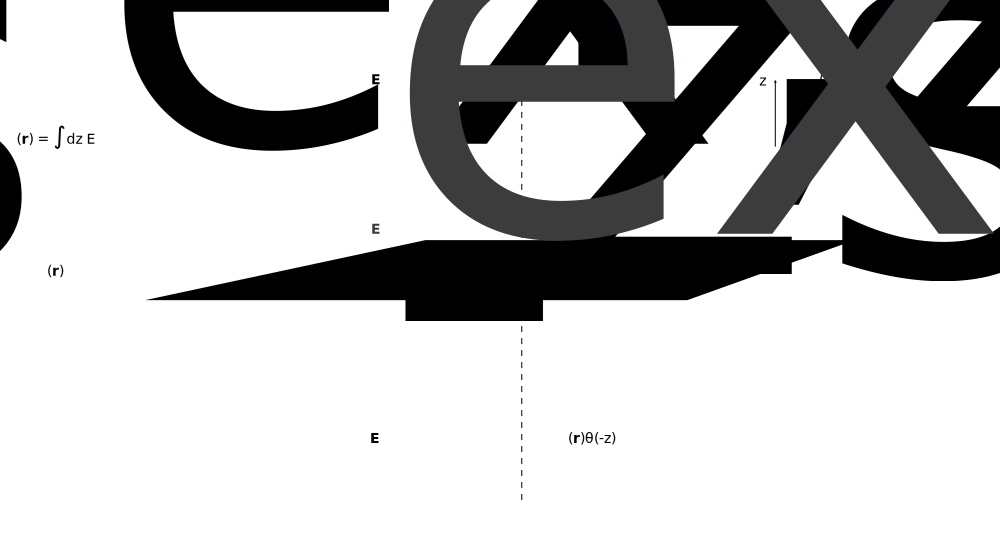
\includegraphics[width=1.0\textwidth]{Figures/excessFields.pdf}
   \caption{The excess fields are integrated over all values of z over the entire surface. Here this 
      is vizualized for the eletric excess field, vizualized by the fog surrounding the surface, as
      the excess field, is only significant close to the surface. Note however that the excess field
      is complicated and not correctly represented by the fog.  (\cite{Lazzari2002}, p.126).
   }
   \label{fig:excessFields}
\end{figure}
%
and gathering them in a singular Dircac term, $\delta(z)$, located at the surface (z=0)
(see Figure \ref{fig:excessFields},
the fields may be rewritten on the form (here shown for just the electric field)
%
\begin{align}
   \label{excessField2}
   \boldsymbol{E}(\boldsymbol{r}) \:=\: \boldsymbol{E}^-(\boldsymbol{r})\theta(-z) 
                                       \:+\: \boldsymbol{E}^s(\boldsymbol{r})\delta(z) 
                                       \:+\: \boldsymbol{E}^+(\boldsymbol{r})\theta(z).
\end{align}
%
Demanding that the fields given by Eq. \eqref{excessField2} fulfill the Maxwell equations 
(\cite{Lazzari2002}, (7-9)) one ends up with the following boundary conditions
%
\begin{subequations}
   \label{exFieldBC} % Excess Field Boundary Conditions
\begin{align}
   \big[ \boldsymbol{E}^+_{\parallel} (\boldsymbol{r}) - \boldsymbol{E}^-_{\parallel} (\boldsymbol{r}) \big] \bigg\rvert _{z = 0} 
       &= i \omega \hat{z} \times \! \boldsymbol{M}^s_{\parallel}(\boldsymbol{r}_{\parallel}) \:-\: \nabla\!_{\parallel} P^s_{z}(\boldsymbol{r}_{\parallel}) 
       \label{exFieldBC1} \\ 
   \big[ D^+_{z} (\boldsymbol{r}) - D^-_{z} (\boldsymbol{r}) \big] \bigg\rvert _{z = 0} 
      &= - \nabla\!_{\parallel} \boldsymbol{P}^s_{\parallel}(\boldsymbol{r}_{\parallel}) 
      \label{exFieldBC2} \\ 
   \big[ \boldsymbol{H}^+_{\parallel} (\boldsymbol{r}) - \boldsymbol{H}^-_{\parallel} (\boldsymbol{r}) \big] \bigg\rvert _{z = 0} 
      &= i \omega \hat{z} \times \! \boldsymbol{P}^s_{\parallel}(\boldsymbol{r}_{\parallel}) \:-\: \nabla\!_{\parallel} M^s_{z}(\boldsymbol{r}_{\parallel})  
      \label{exFieldBC3} \\ 
   \big[ B^+_{z} (\boldsymbol{r}) - B^-_{z} (\boldsymbol{r}) \big] \bigg\rvert _{z = 0} 
      &= - \nabla\!_{\parallel} \boldsymbol{M}^s_{\parallel}(\boldsymbol{r}_{\parallel}), 
      \label{exFieldBC4}  
\end{align}
\end{subequations}
%
which is derived in Vlieger and Bedaux's \textit{Optical Properties of Surfaces} (p.21). 
Here $\nabla_{\parallel}$ is the nabla operator parallel to the surface, while $z$ denotes 
the vector component in the direction normal to the surface at $z = 0$.
In addition, the quantities with superscript $s$ are the so-called excess polarization 
and magnetization densities
\begin{subequations}
\label{surfQuant} %Surface Quantities
\begin{align}
   \boldsymbol{P}^s(\boldsymbol{r}\!_{\parallel}) &= \big( \boldsymbol{D}^s_{\parallel}(\boldsymbol{r}\!_{\parallel}), \:\: - \varepsilon_0 E^s_{z}(\boldsymbol{r}\!_{\parallel}) \big) \label{surfQuant1}\\
   \boldsymbol{M}^s(\boldsymbol{r}\!_{\parallel}) &= \big( \boldsymbol{B}^s_{\parallel}(\boldsymbol{r}\!_{\parallel}), \:\: - \mu_0 H^s_{z}(\boldsymbol{r}\!_{\parallel}) \big) , \label{surfQuant2}
\end{align}
\end{subequations}
Here, in Eq.\eqref{surfQuant}, the quantities on the right hand side
are the integrated excess fields.
%
%PROBLEMS WITH THE NEED FOR CONSTITUTIVE RELATIONS:
%\textit{?? IS THE FOLLOWING CORRECT??} 
%Now, as mentioned above, the excess quantities describe the 
%discontinuitiy in the bulk fields, through the interfacial polarisation and magnetisation desnity,
%$\boldsymbol{P}^s(\boldsymbol{r}_{parallel})$ $\boldsymbol{M}^s(\boldsymbol{r}_{parallel})$. This
%gives the field relations above and below the interface. To explain 
%
%OWN INTERPRETATION: The simplest way to link the surface polarization and magnetization density to the extrapolated bulk fields(?Sigma indexed fields?)involves a
Even though Maxwell's equations have been included, demanding that the fields follow the boundary 
conditions of \eqref{exFieldBC}, they do not uniquely determine the physical situation. 
Maxwell's equations in matter \eqref{ME}, given in Section \ref{sectionFlatScattering}, includes
$\boldsymbol{E}$ and $\boldsymbol{D}$, together with $\boldsymbol{B}$ and $\boldsymbol{H}$, 
, but does not state how they depend on eachother. In other words, Eq. \eqref{ME} does not contain
more information than Maxwell's equations given in free space. So, to fully explain how 
the fields interact with material and the interface, constitutive relations characteristic 
to the surface must be given (like the relations in Eq.\eqref{linearConstitutiveRelations} 
given for the flat interface example) (\cite{Griffiths}, p. 330).
The constitutive relations link the interfacial polarisation and 
magnetization density $\big(\boldsymbol{P}^s(\boldsymbol{r}_{\parallel})$ and 
$\boldsymbol{M}^s(\boldsymbol{r}_{\parallel}) \big)$ and the bulk fields extrapolated to the surface.
%To link the interfacial polarisation and 
%magnetization density, $\boldsymbol{P}^s(\boldsymbol{r}_{parallel})$ and 
%$\boldsymbol{M}^s(\boldsymbol{r}_{parallel})$, and the bulk fields extrapolated to the surface,
%additional relations, which are characteristic to the interface, must be given.
%
If the pertubed surface layer thickness $d$ is negligible compared to the optical wavelength $\lambda$,
the excess fields are only significant or non-negligible close to the surface, which followed
from the notation for the excess fields assumed earlier in Eq. \eqref{excessField1}.
Because of this, the constitutive relations are local and the extrapolated bulk fields may be written on the 
form 
$\boldsymbol{E}_{\parallel, \Sigma} = \big\{ \boldsymbol{E}^+_{\parallel} \!( \boldsymbol{r}\!_{\parallel} ) 
+  \boldsymbol{E}^-_{\parallel} \! (\boldsymbol{r}\!_{\parallel}) \big\} \big/2 $.
For simplisity we restrict our discussion to non-magnetic materials,
i.e. that $\boldsymbol{M}^s(\boldsymbol{r}_{\parallel}) = 0$. The simplest constitutive relation
can be written on the form
\begin{align}
   \boldsymbol{P}^s(\boldsymbol{r}\!_{\parallel}) = \xi ^s_e \: \big[ \boldsymbol{E}_{\parallel, \Sigma}(\boldsymbol{r}\!_{\parallel}), \:\: - D\!_{z, \Sigma}(\boldsymbol{r}\!_{\parallel}) \big].
   \label{constitutiveRel}
\end{align}
By further assuming that the interface is homogeneous and isotropic, the interfacial tensor reduces
to a diagonal matrix:
\begin{align}
  \xi ^s_e = 
\begin{bmatrix}
   \gamma   &   0       &  0      \\
   0        &   \gamma  &  0      \\
   0        &   0       &  \beta 
\end{bmatrix}
,
\end{align}
With the first order surface susceptibilities $\gamma$ and $\beta$. The reason why they are called 
first order susceptibilities is because the discussion above limits the dependence between
the integrated excess quantities and the extrapolated bulk fields to a local relation (second order
would require a spatial relation).
In fact, even though they are not included in this discussion, 
GranFilm also takes account for the non-local dependence, described by the constitutive coefficients of
second order $\delta$ and $\tau$ (\cite{Lazzari2002}, (7,15)). These quantities are of the order
$d/\lambda$ smaller than the first order coefficients. 
Linear combinations of $\delta$ and $\tau$ together with the first order susceptibilities 
$\gamma$ and $\beta$ can construct invariants, which are independent of the choice of the separation surface. 
%
Furthermore, the Fresnel quantities, which all are measurable, are also independent of where we 
choose to put the surface in our coordinate system and can be uniquely expressed as a 
function of these constructed invariants.
This discussion will continue to only consider the first order susceptibilities $\gamma$ and $\beta$,
which are the dominating factors when considering granular layers consisting of metallic islands.




\subsection{The Fresnel coefficients}
Using the same method as for the flat Fresnel surface, the Fresnel coefficients in terms of the surface
susceptibilities can be derived. The derivation is tedious and will not be done here. It can however
be found in Bedeaux and Vlieger's book (\cite{BedeauxVliegerBook}, p.45)  (\cite{LieMaster2010},p.10).
In addition to the classical approach, the excess field boundary conditions \eqref{exFieldBC},
together with the constitutive relation between the interface 
and the extrapolated bulk fields \eqref{constitutiveRel}.
A property of this approach, is that the complicated surface, approximated by the pertubed layer,
does not change the fact of \textit{Snell's law}, which pops out of the boundary conditions
when calculating the classical flat surface problem (\eqref{Griffiths}, p388). In other words, 
\begin{subequations}
\label{snellsLaw}
\begin{align}
   \theta_i &= \theta_r \label{snellsLaw1}\\
   n_{_+} \sin \theta_i &= n_{_-} \sin \theta_t. \label{snellsLaw2}
\end{align}
\end{subequations}
is still used to find the angle of incidence $\theta_i$, reflection $\theta_r$ and transmission $\theta_t$.
They are, so to speak, unmodified by the pertubed layer. However, the Fresnel coefficients, which
decide the reflection and transmission amplitudes, do depend on the pertubed layer through 
the surface susceptibilities. For s-polarization, the resulting Fresnel coefficients are given by
\begin{subequations}
   \label{fresCoeffS}
\begin{align}
   r_s(\omega) &= \frac{n\!_{_-} \cos \theta_i - n\!_{_+} \cos \theta_t + i(\omega/c) \gamma}{n\!_{_-} \cos \theta_i + n\!_{_+} \cos \theta_t - i(\omega/c) \gamma} \label{fresCoeffS1} \\
   t_s(\omega) &= \frac{2 n\!_{_-} \cos \theta_i}{n\!_{_-} \cos \theta_i + n\!_{_+} \cos \theta_t - i(\omega/c) \gamma}. \label{fresCoeffS2}
\end{align}
\end{subequations}
%
For p-polarization the expressions are more complicated
%
\begin{subequations}
\label{fresCoeffP}
\begin{align}
   r_p(\omega) &= \frac{\kappa\!_{_-}(\omega) -i(\omega / c) \gamma \cos \theta_i \cos \theta_t + i(\omega/c)n\!_{_-} n\!_{_+} \varepsilon\!_{_-}\beta\sin^2 \theta_i }
   {\kappa\!_{_+}(\omega) -i(\omega / c) \gamma \cos \theta_i \cos \theta_t - i(\omega/c) n\!_{_-} n\!_{_+} \varepsilon\!_{_-} \beta \sin^2 \theta_i }, \label{fresCoeffP1}\\
   t_p(\omega) &= \frac{2n\!_{_-} \cos \theta_i \big[ 1 + (\omega/2c)^2 \varepsilon\!_{_-} \gamma \beta \sin ^2 \theta_i \big]}
   {\kappa\!_{_+}(\omega) -i(\omega / c) \gamma \cos \theta_i \cos \theta_t - i(\omega/c) n\!_{_-} n\!_{_+} \varepsilon\!_{_-} \beta \sin^2 \theta_i }, \label{fresCoeffP2}
\end{align}
\text{where there has been introduced two quantites $\kappa\!_{_{\pm}}$ defined as}
\begin{align}
   \kappa\!_{_{\pm}} &= \big[ n\!_{_+} \cos \theta _i \pm n\!_{_-} \cos \theta_t  \big]\Bigg[ 1 - \frac{\omega^2}{4c^2} \varepsilon\!_{_-} \gamma \beta \sin ^2 \theta_i \Bigg]. \label{fresCoeffP3}
\end{align}
\end{subequations}
%
%\begin{subequations}
%\begin{align}
   %r_p(\omega) &= \frac{\kappa _-(\omega) -i(\omega / c) \gamma \cos \theta_i \cos \theta_t + i(\omega/c)n_-n_+\varepsilon_-\beta\sin^2 \theta_i }
               %{\kappa _+(\omega) -i(\omega / c) \gamma \cos \theta_i \cos \theta_t - i(\omega/c)n_-n_+\varepsilon_-\beta\sin^2 \theta_i } \\
   %t_p(\omega) &= \frac{2n_- \cos \theta_i \big[ 1 + (\omega/2c)^2 \varepsilon_- \gamma \beta \sin ^2 \theta_i \big]}
               %{\kappa _+(\omega) -i(\omega / c) \gamma \cos \theta_i \cos \theta_t - i(\omega/c)n_-n_+\varepsilon_-\beta\sin^2 \theta_i } \\
   %\kappa_{\pm} &= \big[ n_+ \cos \theta _i \pm n_- \cos \theta_t  \big]\Bigg[ 1 - \frac{\omega^2}{4c^2} \varepsilon_- \gamma \beta \sin ^2 \theta_i \Bigg]
%\end{align}
%\end{subequations}
The simplicity of the expressions for s-polarization \eqref{fresCoeffS} 
compared to p-polarization \eqref{fresCoeffP},
is due to the fact that s-polarized light only manages to excite modes parallel to the surface.
This is reflected in the equations by the fact that $r_s(\omega)$ and $t_s(\omega)$ only depend on the
parallel surface susceptibility $\gamma$.
P-polarized light on the other hand, can excite modes both parallel and perpendicular to the 
interface, and gives rise to the increased complexity of $r_p(\omega)$ and $t_p(\omega)$, with the
dependency of both $\gamma$ and $\beta$. \\
If the surface susceptibilities in the expressions above are set to zero ($\gamma = \beta = 0$),
this means that the perturbation from the flat interface, caused by the granular layer, 
disappears and
the Fresnel coefficients, \eqref{fresCoeffS} and \eqref{fresCoeffP}, reduce to the flat Fresnel 
coefficients, \eqref{flatFresnelCoeffs} and \eqref{flatFresnelCoeffp}, respectively.
\\
\\
In addition to the source frequency $\omega$, the refractive indices $n_{_{\pm}}$ and the incident
angle $\theta_i$ are input parameters. The three latter provide, through Snell's law \eqref{snellsLaw} 
as mentioned above, the calculation of the angle of transmittance $\theta_t$.
However, the surface susceptibilies $\gamma$ and $\beta$ are not known and, 
in order to calculate the Fresnel coefficients for the pertubed surface layer, 
these quantities must be found.

\subsection{Surface susceptibilities of island layer}
To this point, there has been no assumptions regarding the geometrical nature of the surface layer.
The kind of layer to be considered is a discontinuous thin film of nm-sized island, constituting
a granular layer. If the islands are much smaller than the optical wavelength, the 
scattering from the granular film will be negligible and the resulting angular distribution 
of light will be similar to that of a flat interface (\cite{LieL2010}.p.11, (2,p.99) 
\textbf{<- fjern Lie, sjekk og bruk kilde?}).
In this case, the density of islands, or the number of island per unit surface area $\rho$, together with 
their ability to react to the applied field, ,
decide the surface polarization density $\boldsymbol{P}^s(\boldsymbol{r}_{\parallel})$
\begin{align}
   \gamma &= \rho \alpha_{\parallel}         &\beta &= \rho \alpha_{\perp}
\end{align}
The surface's ability to react to the applied field is called the polarizability $\alpha$ of the surface,
where $\alpha_{\parallel}$ is the polarizability parallel to the surface, while $\alpha_{\perp}$
is perpendicular to the surface. (\cite{Lazzari}, (7,11,12,24))
\\
\\
In other words, the optical properties in this situation is essentially driven by the polarizability
of the island. The \textit{GranFilm} software, supports the caulculation of both truncated spheres 
and truncated oblate or prolate spheroids. These two particle shapes can represent a great 
number of experimental situations, with the latter including shapes ranging from discs to needles.
(\cite{Lazzari2002}, p.128)
\\
\\
To calculate the surface polarizabilities, the first step is to solve Laplace's equation for the
electrostatic potential
\begin{align}
   \nabla^2 \Psi(\boldsymbol{r}) = 0
   \label{laplaceEq}
\end{align}
in the quasi-static limit. An easy way to understand the quasistatic limit of Maxwell's equations is,
as stated in (\cite{Larsson2007},p.238), to let $c \rightarrow \infty$, which would neglect all 
effects due to time retardation. This means that any charge or current distribution at any instant in time, 
would decide the resulting fields at the same instant, in all of space. In other words: the effect of 
the sources will be instantaneous. 
The validity of the result depends on the distance to the source
and how fast the fields are fluctuating, making the approximation valid if the distances are
sufficiently short or if the fluctuations of the fields are sufficiently slow
(\cite{Griffiths}, p.308-309).
%\textbf{quasi-static approximation:} In situations where the electric or magnetic fields 
%are changing but electrostatic or magnetoscatic equations are used, the derived results are
%quasi-static and only approximately correct. The validity of the result depends on the 
%distance from the region to the source
%(\textbf{?retardation effects?}) and how fast the fields are fluctuating. If the distances are
%sufficiently short and the fluctuations of the fields are sufficiently slow, the situation is static 
%enough and for a quasi-static approach.
%(\cite{Griffiths}, p.308-309) 
%An easy way to understand the quasistatic limit of Maxwell's equations is, as stated
%in (\cite{Larsson2007},p.238), to let $c \rightarrow \infty$, which would neglect all effects due to time retardation.
%This means that any charge or current distribution at any instant in time, 
%would decide the resulting fields at the same instant, in all of space. In other words: the effect of 
%the sources will be instantaneous.
%
In the case of the granular film, the approximation is valid for sub-wavelength-sized island,
in correspondence to the assumption of the layer thickness compared to the wavelength of the incident
light. \\
Assuming spherical island geometry, the potential can be expanded in a multipolar basis of
seperable solutions to \eqref{laplaceEq}
\begin{align}
   \label{multipoleSolution}
   &\Psi(\boldsymbol{r}) = \sum\limits_{lm} A_{lm} r^{-l-1} Y_l^m(\theta,\phi)
   + \sum\limits_{lm} B_{lm} r^{l} Y_l^m(\theta,\phi)
\end{align}
Here ($r$, $\theta$, $\phi$) are the spherical coordinates centered at the expansion point, 
$A_{lm}$ and $B_{lm}$ are the multipole expansion coefficients and $Y_l^m(\theta,\phi)$ are the
spherical harmonics.
%
\begin{figure}[h!]
  \centering
   \includegraphics[width=1.0\textwidth]{Figures/filmGeometry.pdf}
   \caption{To the left: the transmission and reflection of a pertubed surface layer with thickness $d$, 
      which is assumed to be much smaller than the optical wavelength $\lambda$ of the incoming wave.
      The reflection and transmission amplitudes depend on the surface 
      susceptibilities. The first order surface susceptibilities, $\gamma$ and $\beta$, describe
      the ability of the surface to polarise in the parallel or perpendicular direction. These
      coefficients can be calculated from evaluating the geometry of the trunctated spheres
      (shown to the right), making up
      the granular thin film (\cite{Lazzari2002}, p.126). Adopted from (\cite{Lazzari2002}, p.125)
   }
   \label{fig:filmGeometry}
\end{figure}
%
The coordinate system for the expansion is given in Figure \ref{fig:filmGeometry}, with $\mu$ denoting 
the center of expansion, which may be centered at the truncated sphere or varied along the vertical
symmetry axis. To deal with the boundary truncating the sphere, the classical image technique is used 
(\cite{Lazzari2002},(13)). This is done by having a image expansion center located at 
the opposite side of the surface, compared to $\mu$, inside the substrate.
The image expansion point is denoted by $\bar{\mu}$. 
%
\textbf{Should I also mention $t_r$ and the difference between $t_r > 0$ and $t_r < 0$?}
%
As shown in Figure \ref{fig:filmGeometry}, mathematical approach assumes 4 different media,
even though region 4 is part of the substrate. When specifying the material in the software
region 2 and 4, which constitute the substrate, are usually set to be the same.
Using Eq.\eqref{multipoleSolution} to expand the potential around the expansion center and 
the image, the potential in the different regions take the form:
%
\begin{subequations}
\label{multExp}
\begin{align}
   &\Psi_1(\boldsymbol{r}) = \Psi_i(\boldsymbol{r}) + \sum\limits_{lm}^{l \neq 0} A_{lm} r_{\mu}^{-l-1} Y_l^m(\theta_{\mu},\phi_{\mu})
   + \sum\limits_{lm}^{l \neq 0} A^r_{lm} r_{\bar{\mu}}^{-l-1} Y_l^m(\theta_{\bar{\mu}},\phi_{\bar{\mu}})
   \label{multExp1}\\
%
   &\Psi_2(\boldsymbol{r}) = \Psi_t(\boldsymbol{r}) + \sum\limits_{lm}^{l \neq 0} A_{lm}^t r_{\mu}^{-l-1} Y_l^m(\theta_{\mu},\phi_{\mu})
   \label{multExp2}\\
%
   &\Psi_3(\boldsymbol{r}) = \psi_0(\boldsymbol{r}) + \sum\limits_{lm}^{l \neq 0} B_{lm} r_{\mu}^l Y_l^m(\theta_{\mu},\phi_{\mu})
   + \sum\limits_{lm}^{l \neq 0} B^r_{lm} r_{\bar{\mu}}^l Y_l^m(\theta_{\bar{\mu}},\phi_{\bar{\mu}})
   \label{multExp3}\\
%
   &\Psi_4(\boldsymbol{r}) = \psi_0(\boldsymbol{r}) + \sum\limits_{lm}^{l \neq 0} B_{lm}^t r_{\mu}^l Y_l^m(\theta_{\mu},\phi_{\mu})
   \label{multExp4}
\end{align}
\end{subequations}
%
Here, the $r^l\big|_{l=0}$ terms of the expansion are constant and have been extracted, 
giving the value $\psi_0(\boldsymbol{r})$ inside the sphere (region 3 and 4, see Fig.\ref{fig:filmGeometry}).
The negative terms $r^{-1-l}\big|_{l=0} = r^{-1}$ represents free charge, wich has been assumed to be
zero, and are removed. 
Outside the sphere (region 1 and 2) the potential is set to zero, 
simply because the potential reference point can be chosen freely. 
In addition to the $l=0$-terms, the incident field gives rise to the potential $\Psi_i(\boldsymbol{r})$. 
Some of the incident light is transmitted directly into the substrate and the resulting scalar field
is given by $\Psi_t(\boldsymbol{r})$.
%
\textbf{Burde kanskje ta med at $\Psi_i(\boldsymbol{r})$, $\Psi_t(\boldsymbol{r}) \sim -\boldsymbol{r}\cdot\
\boldsymbol{E}_0$. Men forstår det ikke...(se evt. M.thesis Leif Amind Lie)}
%
Comparing Eqs. \eqref{multExp} to Eq. \eqref{multipoleSolution}, note that all the
$r^l$-terms in region 1 and 2, $r^{-l-1}$-terms in region 3 and 4 are removed due to the divergence
of the potential as $r \rightarrow \infty$ and $r \rightarrow 0$, respectively.
\\
\\
The boundary conditions for the electric potential is given by (\cite{Griffiths}, p.89-90)
\begin{align}
   \varepsilon\!_i\!(\omega) \:\: \partial_n \Psi_i(\boldsymbol{r}) &= \varepsilon\!_j\!(\omega) \:\:\partial_n \Psi\!_j(\boldsymbol{r})
   &\Psi_i(\boldsymbol{r}) &=\Psi\!_j(\boldsymbol{r})
\end{align}
where $\partial_n = \hat{n} \cdot \nabla$ is the derivative with respect to the 
normal direction $\hat{n}$ to the boundary surface, and the indicies $i,j \in \{1,2,3,4\}$, $i \neq j$
denotes the different media included at the different boundaries.
%
From the boundary conditions the relation between the multipole coefficients are found
%
\begin{subequations}
\label{multExpCoeff1}
\begin{align}
   A^r_{lm} & = (-1)^{l+m} \frac{\varepsilon_1 - \varepsilon_2}{\varepsilon_1 + \varepsilon_2} A_{lm}
   \label{multExpCoeffAr}\\
%
   A^t_{lm} & = \frac{2\varepsilon_1}{\varepsilon_1 + \varepsilon_2} A_{lm}
   \label{multExpCoeffAt}
\end{align}
\label{multExpCoeff2}
\begin{align}
   B^r_{lm} & = (-1)^{l+m} \frac{\varepsilon_3 - \varepsilon_4}{\varepsilon_3 + \varepsilon_4} B_{lm}
   \label{multExpCoeffBr}\\
%
   B^t_{lm} & = \frac{2\varepsilon_3}{\varepsilon_3 + \varepsilon_4} B_{lm}.
   \label{multExpCoeffAt}
\end{align}
\end{subequations}
%
However, there are still 4 unknowns for each multipole order (every configuration of $l$ and $m$).
By using the orthogonality of the spherical harmonics $Y_l^m(\theta,\phi)$ to treat the boundary
of the sphere, called the weak formulation of the boundary conditions, give two infinite linear 
systems for the multipolar coefficients $A_{lm}$ and $B_{lm}$ for $l = 1$, $m = 0, \pm 1$.
To solve this system in practive, some cut-off value $l = M$ for the expansion is set. 
Based on investigations by Simonsen and Lazzari \cite{Simonsen2000}
a truncation at $M = 16$ appeared to be sufficient in most cases. This result is based on 
post-checking the boundary condition for the potential and the normal displacement at the surface;
and convergence tests of the first term of the multipolar expansion. Keep in mind, that for 
cases like spherical caps (truncated at the upper hemisphere) or entire spheres on top of a substrate
the convergence could be slower, requiring a truncation $M>16$.
Finally, knowing the first multipolar coefficients the polarizability of the islands can be found
\begin{align}
   \alpha_{\perp} &\simeq A_{10}          &\alpha_{\parallel} &\simeq A_{11}.
\end{align}
The first $l=0$ terms of region 1 $A_{lm}$ are representing the dipole contribution, which dominates
in the far-field limit (\cite{Lie2010}: Bedeaux and Vlieger->(2), \textbf{Må sjekkes!}). 

\subsection{Inter-island coupling; collective contribution}
So far, the discussion has only included the response of a single island and would perhaps 
give resonable result in the low coverage limit. However, this would lead to 
an increase in error for larger covarages and create the need for a correction
due to the increasing island-island interaction (\cite{Lie2010}, p. 20). 
By assuming that the island are sufficiently close to one another such that their mutual separation is 
negligible compared to the optical wavelength, a correction to the low-coverage result can be obtained. 
In this limit, the islands would be excited by the same incident field and have similar responses
to the field. Assuming a dipole response, the islands would be affected by the dipole
fields excited in the neighboring particles. If the spheres are truncated by the substrate through their
lower hemisphere, the modified polarizabilities compared to the isolated polarizatilities, $\alpha_{\perp},
\alpha_{\parallel}$, become
\begin{align}
   \alpha^{\text{mod}}_{\perp} &= \frac{\alpha_{\perp}}{ 1 - 2 \alpha_{\perp} I_{\perp}^{20} }
   &\alpha^{\text{mod}}_{\parallel} &= \frac{\alpha_{\parallel}}{ 1 + 2 \alpha_{\parallel} I_{\parallel}^{20}}.
\end{align}
%
The defined functions in the correction are called the interaction functions
%
\begin{subequations}
\label{couplingPolarizability}
\begin{align}
I_{\perp}^{20} = \frac{1}{\sqrt{20\pi} L^3 \varepsilon_{_-} } 
   \Bigg[
   S_{20} - \Bigg( \frac{\varepsilon_{_-}-\varepsilon_{_+}}{\varepsilon_{_-}+\varepsilon_{_+}} \Bigg) 
   \tilde{S}_{20}^r
   \Bigg]
   \label{couplingPolarizability1}\\
%
   I_{\parallel}^{20} = \frac{1}{\sqrt{20\pi} L^3 \varepsilon_{_-} } 
   \Bigg[
   S_{20} + \Bigg( \frac{\varepsilon_{_-}-\varepsilon_{_+}}{\varepsilon_{_-}+\varepsilon_{_+}} \Bigg) 
   \tilde{S}_{20}^r
   \Bigg],
   \label{couplingPolarizability2}
\end{align}
\end{subequations}
%
where
%
\begin{subequations}
\label{latticeSums}
\begin{align}
   S_{20} = \sum\limits_{i \neq 0} \Bigg( \frac{L}{r}\Bigg)^3 Y_2^0 (\theta,\phi) \Biggr|_{r=R_i}
   \label{latticeSums1} \\
%
   S_{20}^r = \sum\limits_{i \neq 0} \Bigg( \frac{L}{r}\Bigg)^3 Y_2^0 (\theta,\phi) \Biggr|_{r=R_i^r}
   \label{latticeSums2}
\end{align}
\end{subequations}
%
are the direct and image lattice sums, describing the interaction with the other direct and 
image dipoles, respectively. $L$ stands for the lattice constant. The $i=0$ term in the summation
gives the contribution from the interaction with the corresponding image of an island. This 
is taken into account when calculating the isolated response and is therefore not needed in
Eq.\eqref{latticeSums}. 
The validity of the dipolar approximation was tested by Lazzari and Simonsen
for hemispherical silver islands layed out in a hexagonal pattern on a MgO substrate
(\cite{Lazzari2002}, p.129-130). The polarizabilities were computed for $M = 16$ 
and showed that the relative error of the dipole approximation compared quadrupole approximation is
$sim 1\%$ up to 40\% coverage, which is higher than the interesting limits encountered in 
experiments.




















%











the fields above $\boldsymbol{E}^+(\boldsymbol{r})$ and below $\boldsymbol{E}^-(\boldsymbol{r})$ the interface can be calculated for a incident place wave 
(same goes for $\boldsymbol{B}$, $\boldsymbol{D}$ and $\boldsymbol{H}$).
So far, the boundary between the two half-infinite media has been considered to be a sharp, flat discontinuity in $\varepsilon(z)$ and $\mu (z)$. 
As soon as the surface roughness, thickness and/or impurities are taken into acount, the complexity of the problem increases.
\\
\\
\textit{Føler jeg burde ha referance til masteroppgaven jeg har sett på også... er dette en grei ting å gjøre?}







%\textbf{From ''GranFilm-Software-Article''}: \\
%Information on the dieletric behavior of surfaes can often be obtained by measuring the Fresnel coefficients,
%such as reflection, transmission and absorption. \\
%?p.2?: for a layer with thickness negligible compared to wavelength, we introduce surface susceptibilities 
%which interconnect the  fresnel coeff. and characterise the optical response of the surface. ?? DID I UNDERSTAND THIS CORRECTLY? ?? \\
%Since all the Fresnel coeff. can be expressed in terms of these surface susceptibilities, the main task consist of calculating these coefficients for the appropriate geometry. \\
%\textbf{Goal of GranFilm:} to calculate ?surface-susceptibility-/fresnel-coefficients? and the associated measurableFresnel quantities for various surface layer geometries. 
%\begin{itemize}
%\item GranFilm is free open-source software
%\end{itemize}
%\subsection{Mie resonances/ plasmon absorption modes}
%\textbf{From ''GranFilm-Software-Article''}: \\
%when small metallic particles, the resonances can be absorbed by visible light and strongly affect the fresnel 
%coefficients depending on the particle morphology.
%%
%\subsection{Quasistatic Approximation}
%%
%\subsection{Electromagnetic excess fields }
%%
%\textbf{From ''GranFilm-Software-Article''}: \\
%(Bedeaux and Vlieger) \\
%Difference between the bulk extrapolated fields and the real fields. The BC at the dividing surface
%(which drive all fresnel coeff.) are given in terms of the integrated excess fields perpendicular to
%the surface. \\
%Bedeaux and Vlieger $\rightarrow$ formalism of excess quantities (does not require exact knowledge of the near suface EM-field behaviour). \\
%Excess fields are defined as the differene between the real fields and the bulk fields extrapolated to the surface. E.g. for the electric field $E(r)$ the excess quantity is defined as
%\begin{align}
   %E_{ex} (r) = E(r) - E^-(r) \theta(-z) - E^+(r)\theta(z),
%\end{align}
%where $\theta(z)$ is the Heaviside function and the superscript $\pm$ are used to indicate the region above (+) and below (-) the dividing interface at $z = 0$. 
%The excess field is only significant close to the surface, since $E(r, \omega) \rightarrow \rightarrow E^{\pm}(r,\omega)$  for $z \rightarrow \pm \infty$. \\
%\textit{QUESTION: \@ Is the $E^{\pm}$ field solved for a infinite homogeneous medium of type (+) and (-) respectively  OR the field in simple two media interface scattering?} \\
%\textbf{From Leif Amund Lies Msc Thesis}: \\
%Since the excess fields will only be significant close to the surface, they may be thought of as perturbations to the simple case of flat interface. 
%\textit{OWN INTERPRETATION: \@ This meas that the bulk fields are the fields created from scattering in the interface between two half-infinite media.} \\
%Instead of tediously using the quasi-static-"no source"-BC, the excess fields defined as for the electric field above are inserted into the full Maxwell equations to derive new non-sharp boundary conditions.
%The result reads
%%
%\textbf{From Leif Amund Lies Msc Thesis AND GranFilm-Article}: \\










\begin{thebibliography}{9}

      \bibitem{Lazzari2002}
      Lazzari R, Simonsen I. 
      GranFilm: a software for calculating thin-layer 
      dielectric properties and Fresnel coefficients.
      Thin Solid Films 
      2002;419:124-136
      \textit{ER DETTE RIKTIG?}

      \bibitem{Griffiths}
      Griffiths DJ.
      Introduction to electrodynamics, third edition.
      Pearson, international edition 2008.
      
      \bibitem{BedeauxVliegerBook}
      Bedeaux D, Vlieger J. 
      Optical properties of surfaces. 
      Imperial College Press, second edition 2004.

      \bibitem{Larsson2007}
      Larsson J.
      Electromagnetics from a quasistatic perspective.
      American Association of Physics Teachers, 2007.
      \textbf{??Er denne riktig???}

      \bibitem{Simonsen2000}
      Simonsen I, Lazzari R. Jupille J, Roux S.
      Numerical modeling of the optical response of supported metallic particles.
      Physical Review B, 61(11):7722-7733, 2000.


      \bibitem{LieMaster2010}
      Lie LA, Simonsen I.
      Optical properties of a thin film of coated, truncated spheres.
      NTNU 2010.
      Imperial College Press, second edition 2004.
\end{thebibliography}
